\section{Задание №10}

Провести фильтрацию одномерного процесса Орнштейна--Уленбека:
\begin{enumerate}
        \item Используя генератор белого шума, добавить случайную ошибку с известной дисперсией к реализации процесса Орнштейна--Уленбека.
        \item При помощи фильтра Калмана оценить траекторию процесса по зашумленному сигналу. Параметры процесса и белого шума считать известными.
        \item Рассмотреть случай, когда шум 
        \begin{itemize}
                \item является гауссовским,
                \item имеет распределение Коши.
        \end{itemize}
\end{enumerate}


\subsection{О белом шуме}

\begin{definition}
        \textit{Дискретным белым шумом} называется последовательность $\{\varepsilon_k\}_{k=1}^{\infty}$ независимых одинаково распределенных случайных величин.
\end{definition}

Рассмотрим соотношение
$$
        x_{k+1} = f(x_k) + \omega_k,
$$
где $\omega_k$ --- случайная помеха, $x_k,\,\omega_k$ независимы, а $f(x_k) = \E(x_{k+1}\,|\,x_{k})$. Пусть рассматривается марковский процесс, тогда 


\subsection{Фильтр Калмана для гауссовского шума}

Рассмотрим следующую систему:
$$
        \begin{cases}
x_{k+1} = A_k x_k + w_k, \\
y_{k+1} = C_{k+1}x_{k+1} + v_{k+1}.
        \end{cases}
$$
Здесь $x_0, w_0, \ldots, w_{N-1}, v_0,\ldots,v_{N-1}$ независимые в совокупности случайные величины. $Y_{N-1} = (y_0,\ldots,y_{N-1})^\T$ --- все наблюдения, а $X_{N-1} = (x_0,\ldots,x_{N-1})$ --- исходный процесс, который надо найти. Для этого воспользуемся фильтром Калмана, а точнее его схемой ,,шагаем мерим``, общий вид которой совпадает с вышеприведенной системой.

Фильтр Калмана для схемы ,,шагаем мерим`` имеет вид:
$$
        \begin{cases}
x_{k+1|k} = A_k x_{k|k},
        \\
x_{k+1|k+1}
=
x_{k+1|k}
+
R_{k+1|k}
C_{k+1}^\T
(
        C_{k+1}
        R_{k+1|k}
        C_{k+1}^\T
        +
        N_{k+1}
)^{-1}
(
        y_{k+1}
        -
        C_{k+1}
        x_{k+1|k}
),
        \\
R_{k+1|k}
=
A_k
R_{k|k}
A_k^\T
+M_k,
        \\
R_{k+1|k+1}
=
R_{k+1|k}
-
R_{k+1|k}
C_{k+1}^\T
(
        C_{k+1}
        R_{k+1|k}
        C_{k+1}^\T
        +
        N_{k+1}
)^{-1}
C_{k+1}
R_{k+1|k},
        \\
x_{0|0} = \E\,x_0,
        \\
R_{0|0} = \Var\,x_0.
        \end{cases}
$$
\begin{remark}
        Нам действительно достаточно рассматривать только первые и вторые моменты, потому что исследуемый случайный процесс имеет гауссовское распределение, а значит полностью определяется этими величинами.
\end{remark}

В нашей задаче $x_k$ --- процесс Орнштейна--Уленбека с параметрами $\sigma$ и $\lambda$, $y_{k+1} = x_{k+1} + v_{k+1}$. То есть сразу имеем, что $C = 1$, а $N_k$ --- дисперсия белого шума (обозначим эту дисперсию за $\sigma^2_v$).

В системе нам пока неизестны величины $A_k$ и $M_k$. Найдем их. Для начала условимся, что $t_{k+1} - t_k = \Delta t$ постоянная величина для каждого испытания. Тогда с одной стороны мы имеем
$$
        \Var\,x_{k+1}
        =
        A^2_k \Var\,x_k
        +
        \Var\,w_k
        =
        A^2_k \Var\,x_k + M_k,
$$ 
\begin{multline*}
        \mathrm{cov}(x_{k+1},\,x_k)
        =
        \E(x_{k+1}x_k)
        -
        \E\,x_{k+1}
        \E\,x_k
        =
        \E(X_k x_k^2 +w_{k+1}x_k)
        -
        A_k(\E\,x_k)^2
        =\\=
        \{\;\mbox{$\E\,w_{k+1} = 0$, $w_{k+1}$ и $x_k$ независимы}\;\}
        =
        A_k(\E\,x_k^2 - (\E\,x_k)^2)
        =
        A_k\Var\,x_k.
\end{multline*}
\begin{remark}
        Здесь и далее считаем распределение помехи $v$ гауссовским. В случае распределения Коши матожидание помехи не определено и фильтрацию получить не получится.
\end{remark}

С другой стороны мы знаем ковариационную функцию процессса Орнштейна--Уленбека $R(t,s) = \sigma^2e^{-\lambda|t-s|}$. Это дает нам следующую систему:
$$
        \begin{cases}
A_k^2 \Var\,x_k + M_k = \sigma^2,
        \\
A_k \Var\,x_k = \sigma^2 e^{-\lambda\Delta t},
        \\
\Var\,x_k = \sigma^2.
        \end{cases}
$$
Как итог получаем все необходимые значения:
$$
        A_k = e^{-\lambda \Delta t}
\quad
\mbox{и}
\quad
        M_k = \sigma^2\left(1- e^{-2\lambda\Delta t}\right).
$$

Собирая все вместе, получаем фильтр Калмана для нашей задачи:
$$
        \begin{cases}
x_{k+1|k}
=
e^{-\lambda\Delta t} x_{k|k},
        \\
x_{k+1|k+1}
=
x_{k+1|k}
+
R_{k+1|k}
(
        R_{k+1|k}
        +
        \sigma^2_v
)^{-1}
(
        y_{k+1}
        -
        x_{k+1|k}
),
        \\
R_{k+1|k}
=
e^{-2\lambda\Delta t}
R_{k|k}
+\sigma^2(1 - e^{-2\lambda\Delta t}),
        \\
R_{k+1|k+1}
=
R_{k+1|k}
-
R_{k+1|k}
(
        R_{k+1|k}
        +
        \sigma^2_v
)^{-1}
R_{k+1|k},
        \\
x_{0|0} = 0,
        \\
R_{0|0} = \sigma^2.
        \end{cases}
$$


\clearpage
\begin{figure}[t]
        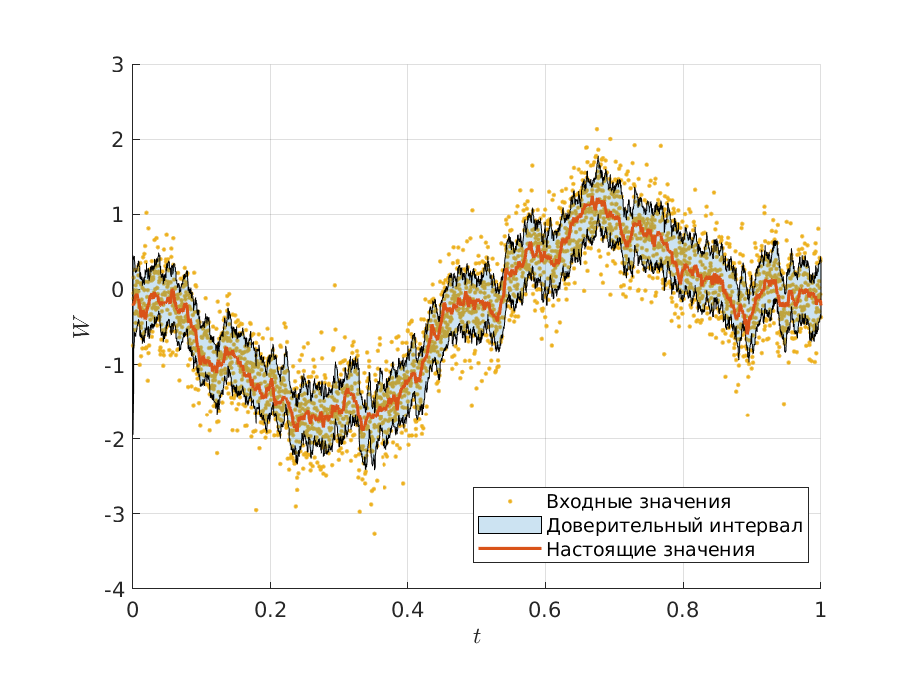
\includegraphics[width=0.5\linewidth]{task_10/n_big.eps}
        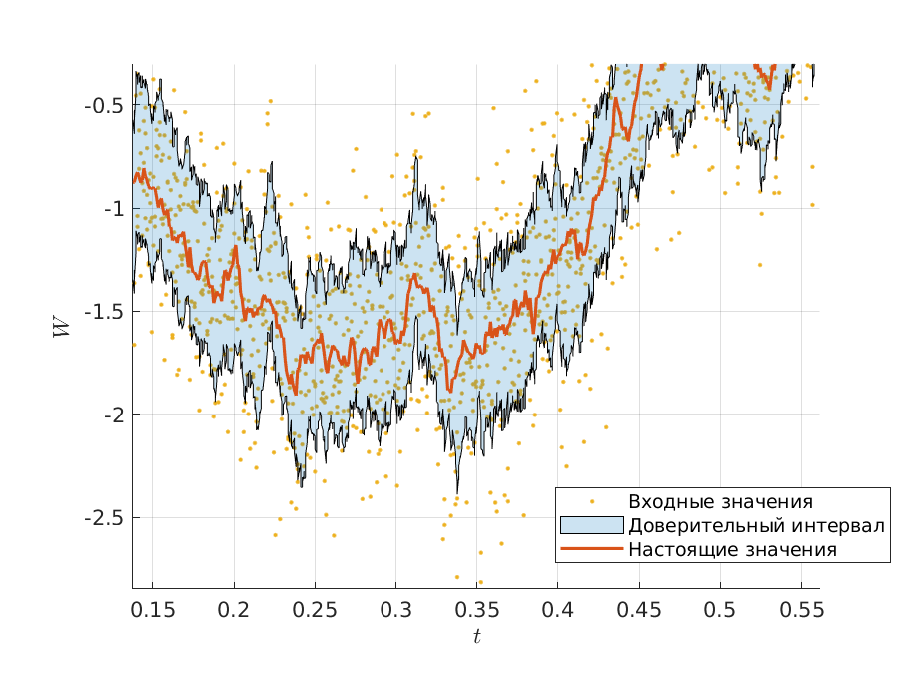
\includegraphics[width=0.5\linewidth]{task_10/n_small.eps}
        \caption{Демонстрация работы фильтра Калмана для гауссовского шума с параметрами распределения $\mu = 0$, $\sigma^2 = 0.4$ на всем отрезке (слева) и приближенно (справа).}
\end{figure}
\begin{figure}[b]
        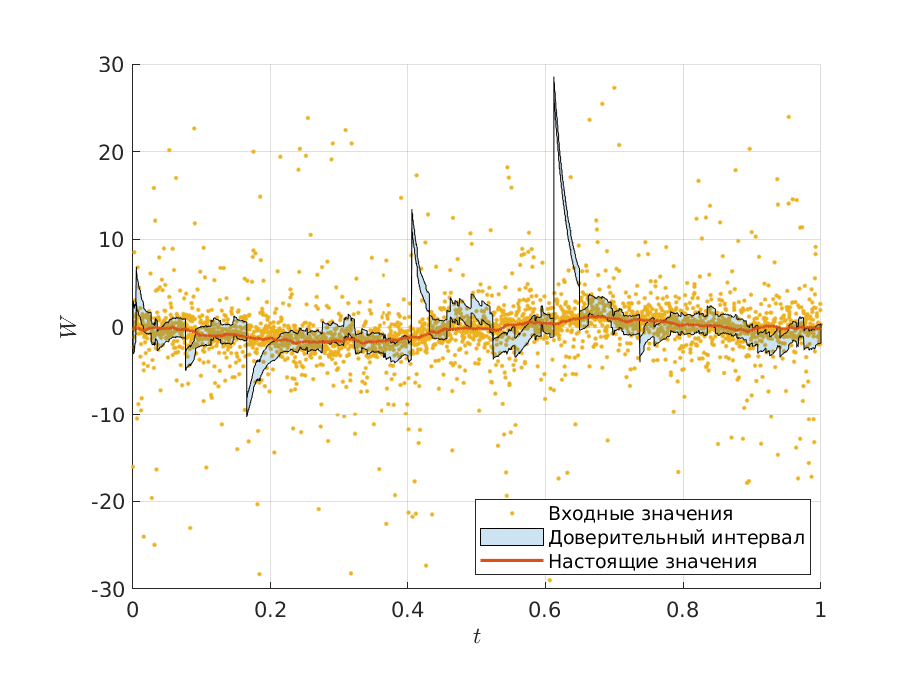
\includegraphics[width=\linewidth]{task_10/c.eps}
        \caption{Демонстрация работы фильтра Калмана для шума с распределением Коши с параметрами $a = 0$, $b = 1$. Видно, что фильтр Калмана не подходит для избавления от шумов, у которых не определено математическое ожидание.}
\end{figure}